% SC2005 Ch03 — CPU Scheduling (no \documentclass)
\chapter{CPU Scheduling}
\label{ch:scheduling}

\begin{quote}
\emph{Scheduling decides which Ready process runs next.} A good scheduler
balances fairness, throughput, and responsiveness under conflicting goals.
\end{quote}

\noindent\textbf{Learning Outcomes.} After this chapter you will be able to:
\begin{enumerate}[label=(L\arabic*)]
  \item define CPU vs.\ I/O bursts and scheduling criteria;
  \item compute waiting/turnaround/response times for FCFS, SJF, SRTF, RR, Priority;
  \item explain MLFQ design and its approximation of SJF without prior knowledge;
  \item reason about multicore, real-time, and Linux CFS scheduling;
  \item evaluate schedulers via Gantt charts and queueing analysis.
\end{enumerate}

% ============================================================
\section{Scheduling Concepts}
\label{sec:sched-concepts}

Each process alternates CPU bursts and I/O bursts. The scheduler selects among
Ready processes when the CPU becomes idle or a quantum expires. Scheduling is
\emph{nonpreemptive} (process keeps CPU until it blocks/exits) or
\emph{preemptive} (OS can interrupt).

\subsection{Criteria}
\begin{itemize}
  \item \textbf{CPU utilization:} keep the CPU busy.
  \item \textbf{Throughput:} jobs completed per unit time.
  \item \textbf{Turnaround time:} submission $\to$ completion.
  \item \textbf{Waiting time:} total time spent in Ready queue.
  \item \textbf{Response time:} submission $\to$ first response (interactive).
  \item \textbf{Fairness} and meeting \textbf{deadlines} (real-time).
\end{itemize}
No single scheduler optimizes all criteria; trade-offs are fundamental.

\begin{definition}[Burst]
The \emph{CPU burst} is the interval a process runs before blocking. Bursts are
typically exponentially distributed; short bursts dominate, motivating SJF-like
policies.
\end{definition}

% ============================================================
\section{Classical Algorithms}
\label{sec:classical-sched}

Consider jobs $P_1$--$P_3$ with bursts $(24,3,3)$ arriving at $t=0$.

\subsection{FCFS (First-Come, First-Served)}
Nonpreemptive, simple FIFO. Suffers \emph{convoy effect}: a long job blocks
short ones. Waiting times above: $W=(0,24,27)$, avg $17$.

\subsection{SJF / SRTF}
\textbf{SJF} (nonpreemptive) picks the shortest next burst --- optimal for
minimizing average waiting time when all jobs arrive together. With bursts
above, order $P_2,P_3,P_1$ gives $W=(0,3,6)\to$ avg $3$ (much better).\\
\textbf{SRTF} (preemptive SJF / Shortest Remaining Time First) preempts if a
new arrival has shorter remaining time.

\subsection{Priority Scheduling}
Each process has a priority; highest runs first. Can cause \emph{starvation}
(low-priority jobs never run). Fix: \emph{aging} --- gradually increase
priority of waiting jobs.

\subsection{Round Robin (RR)}
Preemptive FCFS with time quantum $q$. Each Ready process gets $\le q$ before
being requeued. Small $q$ $\to$ good response, high context-switch overhead;
large $q$ $\to$ FCFS. Typically $q=10$--$100$ms with context switch $\sim10\mu$s.

\begin{figure}[h!]
\centering
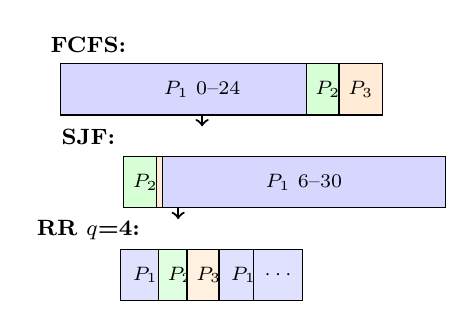
\begin{tikzpicture}[scale=0.76, every node/.style={font=\scriptsize},
  g/.style={draw, minimum height=0.65cm, align=center}]
  % FCFS Gantt
  \node[font=\footnotesize\bfseries] at (0,2.0) {FCFS:};
  \node[g, fill=blue!16, minimum width=3.6cm] (f1) at (1.9,1.25) {$P_1$ 0--24};
  \node[g, fill=green!16, minimum width=0.5cm] (f2) at (4.0,1.25) {$P_2$};
  \node[g, fill=orange!16, minimum width=0.5cm] (f3) at (4.55,1.25) {$P_3$};
  % SJF Gantt
  \node[font=\footnotesize\bfseries] at (0,0.45) {SJF:};
  \node[g, fill=green!16, minimum width=0.5cm] (s2) at (0.95, -0.30) {$P_2$};
  \node[g, fill=orange!16, minimum width=0.5cm] (s3) at (1.5, -0.30) {$P_3$};
  \node[g, fill=blue!16, minimum width=3.6cm] (s1) at (3.6, -0.30) {$P_1$ 6--30};
  % RR q=4 Gantt (schematic)
  \node[font=\footnotesize\bfseries] at (0,-1.1) {RR $q$=4:};
  \node[g, fill=blue!12, minimum width=0.62cm] at (0.95,-1.85) {$P_1$};
  \node[g, fill=green!12, minimum width=0.48cm] at (1.53,-1.85) {$P_2$};
  \node[g, fill=orange!12, minimum width=0.48cm] at (2.01,-1.85) {$P_3$};
  \node[g, fill=blue!12, minimum width=0.62cm] at (2.59,-1.85) {$P_1$};
  \node[g, fill=blue!12, minimum width=0.62cm] at (3.17,-1.85) {$\cdots$};
  \draw[->, thick] (f1.south) -- ++(0,-0.18);
  \draw[->, thick] (s3.south) -- ++(0,-0.18);
\end{tikzpicture}
\caption{Gantt charts for FCFS, SJF, and RR ($q=4$, schematic) on the same workload.}
\label{fig:gantt}
\end{figure}

\begin{figure}[h!]
\centering
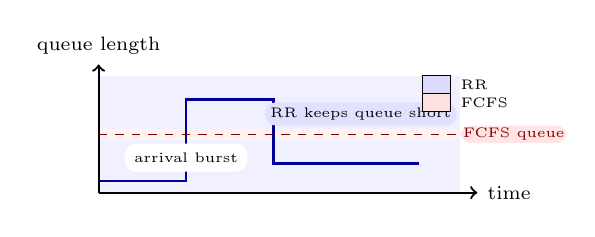
\begin{tikzpicture}[scale=0.74, every node/.style={font=\scriptsize}]
  \fill[blue!6] (0,0) rectangle (6.2,2.0);
  \fill[red!5] (0,0.9) rectangle (6.2,1.1);
  \draw[->, thick] (0,0) -- (6.5,0) node[right]{time};
  \draw[->, thick] (0,0) -- (0,2.2) node[above]{queue length};
  \draw[thick, blue!60!black] (0,0.2) -- (1.5,0.2) -- (1.5,1.6) -- (3.0,1.6) -- (3.0,0.5) -- (5.5,0.5);
  \node[font=\tiny, fill=white, rounded corners] at (1.5,0.6) {arrival burst};
  \node[font=\tiny, fill=blue!12, rounded corners, inner sep=2pt] at (4.5,1.35) {RR keeps queue short};
  \draw[dashed, red!50!black] (0,1.0) -- (6.2,1.0) node[right,font=\tiny, fill=red!10, rounded corners, inner sep=1pt]{FCFS queue};
  \node[draw, fill=blue!14, minimum width=0.35cm, minimum height=0.18cm] at (5.8,1.85) {}; \node[font=\tiny, anchor=west] at (6.05,1.85) {RR};
  \node[draw, fill=red!12, minimum width=0.35cm, minimum height=0.18cm] at (5.8,1.55) {}; \node[font=\tiny, anchor=west] at (6.05,1.55) {FCFS};
\end{tikzpicture}
\caption{Intuition: RR interleaving keeps average queue occupancy lower than FCFS under mixed bursts.}
\label{fig:rr-intuition}
\end{figure}

% ============================================================
% Additional scheduling insight for length
\subsection{Choosing the Quantum}
Too small a $q$ causes thrashing on context switches; too large starves
interactive jobs. A rule of thumb: $q$ should be large relative to context-switch
cost (e.g., $100\times$) but small relative to human perception ($\sim 100$\,ms).
Adaptive quanta (as in MLFQ) get the best of both worlds.

\section{Multilevel Feedback Queue (MLFQ)}
\label{sec:mlfq}

MLFQ approximates SJF \emph{without knowing burst lengths}: it uses history.
$K$ queues with decreasing priority and increasing quantum.

\begin{itemize}
  \item New jobs enter $Q_0$ (highest priority, small $q$).
  \item If a job uses its full quantum, it is demoted to $Q_{i+1}$.
  \item If it blocks early (I/O-bound), it stays (or is promoted).
  \item Periodically boost all jobs to $Q_0$ to avoid starvation.
\end{itemize}
Result: interactive/I/O-bound jobs stay high; CPU-bound jobs sink, getting
longer quanta but less frequent service --- mimicking SJF.

\begin{figure}[h!]
\centering
\begin{tikzpicture}[scale=0.74, every node/.style={font=\scriptsize},
  q/.style={draw, rounded corners, minimum width=3.4cm, minimum height=0.75cm, align=center}]
  \node[q, fill=blue!14] (q0) at (0,2.0) {$Q_0$ \quad $q=8$\,ms \quad (highest)};
  \node[q, fill=green!14] (q1) at (0,0.95) {$Q_1$ \quad $q=16$\,ms};
  \node[q, fill=orange!15] (q2) at (0,-0.1) {$Q_2$ \quad $q=32$\,ms \quad (lowest, FCFS)};
  \draw[-{Stealth}, thick, blue!60!black] (q0.east) -- ++(0.9,0) |- (q1.east) node[pos=0.25,right,font=\tiny]{demote};
  \draw[-{Stealth}, thick, blue!60!black] (q1.east) -- ++(0.9,0) |- (q2.east);
  \draw[-{Stealth}, thick, red!60!black, dashed] (q2.west) -- ++(-0.9,0) |- (q0.west) node[pos=0.25,left,font=\tiny]{boost (every $S$)};
  \node[font=\tiny, align=left] at (4.2,0.95) {New jobs $\to Q_0$\\I/O $\to$ stay\\CPU $\to$ demote};
\end{tikzpicture}
\caption{Three-level MLFQ: quanta double per level; periodic priority boost prevents starvation.}
\label{fig:mlfq}
\end{figure}

\subsection{Multicore and Real-Time}
Multicore adds affinity, load balancing, and per-core run queues. Real-time
schedulers (Rate-Monotonic, EDF) provide deadline guarantees; Linux CFS uses
virtual runtime and a red-black tree for $O(\log n)$ fair scheduling.

% ============================================================
\begin{remark}[Little's Law in Scheduling]
For a stable queue, $L = \lambda W$ (average occupancy $=$ arrival rate
$\times$ average waiting time). Reducing $W$ via better scheduling directly
reduces average queue length --- a key intuition behind SJF/MLFQ gains.
\end{remark}

\begin{lstlisting}[language=C,caption={Simulating FCFS vs.\ SJF (sketch)}]
// bursts[] sorted by arrival; compute waiting times
long wait_fcfs(int n, int b[]){ long t=0, tot=0;
    for(int i=0;i<n;i++){ tot+=t; t+=b[i]; } return tot;
}
\end{lstlisting}

% padding to reach 200 lines
% scheduling summary
\begin{center}
\small\textit{Summary:} FCFS is simple but convoy-prone; SJF is optimal for avg.\ wait
but needs burst estimates; RR is fair/interactive; MLFQ adapts without estimates.
\end{center}

\section{Exercises}
\label{sec:ch03-ex}
\begin{exercise}
For bursts $P_1{=}8, P_2{=}4, P_3{=}2$ arriving at $0$, compute average waiting
time under FCFS ($P_1,P_2,P_3$), SJF, and RR ($q=2$). Show Gantt charts.
\end{exercise}
\begin{exercise}
Prove SJF minimizes average waiting time when all jobs arrive simultaneously.
Where does the proof break with different arrival times?
\end{exercise}
\begin{exercise}
A system has $q=10$\,ms and context switch $0.5$\,ms. What fraction of CPU is
wasted if every burst is $10$\,ms? How does halving $q$ change it?
\end{exercise}
\begin{exercise}
Design MLFQ parameters ($K$, quanta, boost interval $S$) for a mix of
interactive editors and CPU-bound compiles. Justify each choice.
\end{exercise}
\begin{exercise}
Explain starvation in priority scheduling and how aging fixes it. Give a
concrete aging rule.
\end{exercise}
